\documentclass{article}
\usepackage{tikz}
\usepackage{amsmath}
\usepackage{graphicx}
\usetikzlibrary{positioning}
\usepackage{float}
\usepackage{adjustbox}
\usepackage{amsfonts}
\newcommand{\Z}{\mathbb{Z}}
\DeclareMathOperator*{\minimize}{minimize}
\DeclareMathOperator*{\subjectto}{s.t}
\title{Project 2, Part 2\\ Branch and Bound solutions for MILPs}
\author{Matt Kingsinger, Hongjun Choi, Adarsh Akkshai}
\begin{document}
\maketitle

\begin{itemize}
\item[[1-d]] The program IP1.m solves an MIP by recursively calling the function rec() which leads to a depth-first search of every branch in the Branch-and-Bound solving 
strategy. In our own words we describe how IP1.m works:
\vspace{.2in}

It first uses linprog function to solve the MILP without the integrality constraints, this gives an initial solution to the relaxed MILP. We then send this
initial solution to the function rec along with all of the vectors and matrixes that define our original MILP. Within IP1.m the bulk of the work is done by recursively calling [x,val,status,b]=rec(f,A,b,Aeq,beq,lb,ub,x,v,M,e,bound). Here is an explanation of the variables that are passed to rec():

\textbf{f:} represents the objective function

\textbf{A and b:} represent the inequality contraints

\textbf{Aeq and beq:} represent the equality contraints

\textbf{lb and ub:} represent the bounds for each variable

\textbf{x, v:} the initial relaxed solution and objective value

\textbf{M:} a vector holding the indeces of the variables in our solution vector x that must be integers

\textbf{e:} the amount from a true integer value that we will allow for our integral variables

\textbf{bound:} a number that we require our objective be less than
\vspace{.2in}

If the relaxed MILP returned by linprog has either status0 < 0 or
        val0 > bound (note that the minimal solution for the relaxed LP
        is lower bound for the minimal solution to the MILP), then the
        MILP cannot be sufficientl solved. We then return the solution,
        objective, status, and bound for the relaxed LP and our optimization
        ends.
\vspace{.1in}

Otherwise, we test to see if the returned "relaxed" solution satisfies
        our requirements and is in fact an MILP solution (line 54). If it is,
        and the objective $val0 < bound$, then we return this as the MILP
        solution, AND WE SET bb = val0 (This will be critical in our comparing of answers
        returned by the recursive calls for A1, b1 and A2, b2). If $val0 \geq bound$, then return the relaxed LP solution. We
        were not able to find a satisfactory MILP solution.
\vspace{.1in}

If the solution to the relaxed LP exists and is satisfactory, but it is
        not an integral solution, then we proceed with the rec() function
        to do depth-first branch and bound until we find an integral solution.
\vspace{.1in}

ind is a vector containing all of the indices for the elements of M (which)
        correspond to the variables of our solution x0 which do not satisfy
        the integerality requirement. We will work branch on the first element
        of ind.
\vspace{.1in}

The algorithm builds matrix A1 to be the same as A with one more row of
        zeros, and the vector b1 to be the same as b with a zero entry added.
        Then it places a 1 in the last row at the column corresponding to the
        variable br\_var = M(ind(1)) in our solution x0 for which we are branching. In the added
        zero entry of b1 it places the value of floor(x(br\_var)). This adds one inequality to our contraints
        which is equivalent to the less-than branch of our node. Similarly A2 and b2 are created to simulate adding
        an inequality to our original contraints that represents the greater-than branch of the node [done by using a $<$ inequality
        operated on the negative of ceiling(x(br\_var))].
\vspace{.1in}

We first recursivly solve the MILP with A1 and b1 and check if we recieve a satisfactory solution If we do then we set xx, val, and bound
        equal to the returned bb. Then we do the same recursive call with A2 and b2. If we are returned a status the is $>0$ then we have found a
        feasible solution to the MILP somewhere along the greater-than branch. We check if $bound2 < bound$ (which may be bound = bound1 if the
        less-than branch returned a feasible MILP solution). If $bound2 < bound$ then we return the solution found along the greater-than branch.
        Either way we have used the recursive function to do a depth-first search of every branch of the tree, hence we have found the optimal
        MILP solution, if one exists.
\vspace{.2in}

\begin{figure}[htp!]
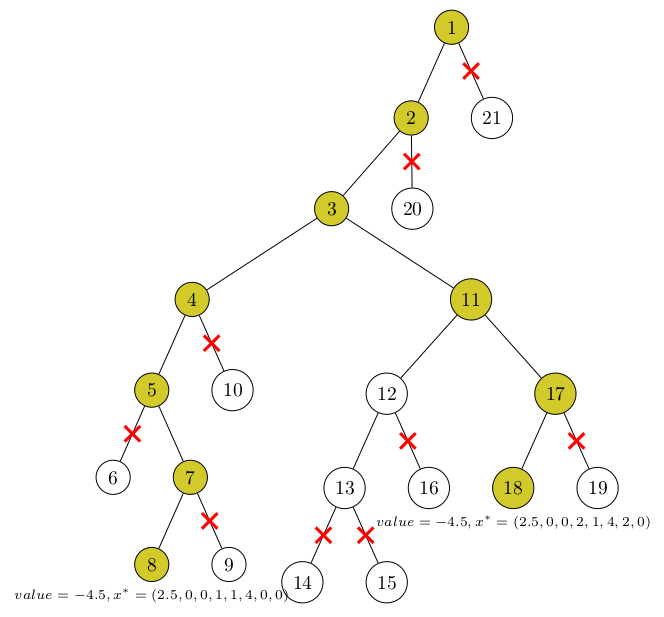
\includegraphics[scale=.5]{prob1d_matlab_depthfirst}
\caption{The nodes expanded in Depth-first Branch-and-Bound search (see explanation on next page)}
\vspace{.5in}
\begin{center}
(See \textbf{Run.m} and \textbf{Run\_matlab\_output.txt})
\end{center}
\end{figure}

\newpage

The result of Depth-first Branch-and-Bound algorithm is shown in Fig 1. The goal nodes are yellow circle, numbered "8" and "18". In the algorithm, suppose initial bound=infinity and the depth-first search always chooses the leftmost node first. Above figure shows the order in which the nodes are checked to determine if they are a goal node. The edges that are with a red 'X'  are infeasible solutions. 

The eighth node checked is a goal node. Hence, the current bound is substituted for the bound of node numbered  "8". From then on, only bounds with the value of less then the bound of "8" are checked for being optimal solution. 
The subtree under the node numbered "12" does not have a goal and is explored fully. As we can see at this node, the interesting point at time is that depth-first algorithm does not always guarantee best path to the goal node since the nodes that numbered "14" and "15" could not be feasible solutions. 
The eighteenth node checked is also a goal node and it has path length of 5 with value of the objective function -4.5 as like at node "8". This is an optimal path and so the path to the node labeled "18" is returned.

\newpage

We have created a more interesting MILP for IP1.m to solve (See \textbf{coolmilp.lp} and \textbf{coolmilp.m}.) 
\vspace{.2in}

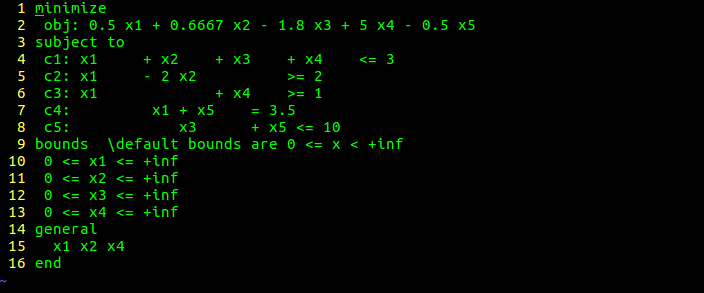
\includegraphics[scale=.5]{coolmilp}

\vspace{.2in}

See \textbf{coolmilp\_LP\_output.txt} for the CPLEX solution of the problem and \textbf{coolmilp\_matlab\_output.txt} for the solution given by the matlab code IP1.m. Notice that they are equivalent. 
    
\newpage

\item[[1-e]] Explanation of FEASPUMP algorithm:
\vspace{.2in}

In our MILP the solution $x^*$ will need to have certain components $x_j\in \mathbb{Z}$. We define $I = \{j|x_j\in \mathbb{Z}\}$. The FEASPUMP algorithm works by building two sequences that have at most $K$ terms (K is chosen by the user):
\vspace{.1in}

$\{\overline{x}_k\}_{k=1}^K$ \hspace{1.0in} noninteger solutions to "relaxed" MILP
\vspace{.1in}

$\{\tilde{x}_k\}_{k=1}^K$ \hspace{1.0in} integer, but possibly non-feasible for MILP
\vspace{.1in}

%$\{\overline{x}_k\}_{k=1}^K$ \hspace(1.0in} integer, but possibly non-feasible for MILP
FEASPUMP begins this process by taking our MILP and relaxing the integrality constraints (making it an LP). It then solves the LP giving us an initial "relaxed" MILP solution $\overline{x}_1$. For each component of the solution $\overline{x}_1$ that is not integer, but needs to be integer based upon the MILP constraints, FEASPUMP rounds to the nearest integer. Hence, from $\overline{x}_1$ we get $\tilde{x}_1$:
\[
\overline{x}_1 \rightarrow (round) \rightarrow \tilde{x}_1.
\]  
If $\tilde{x}_1$ is a feasible solution to the MILP, then we are done and FEASPUMP returns this solution. If $\tilde{x}_1$ is NOT a feasible solution, then FEASPUMP begins a search for the next term, $\overline{x}_2$, in the sequence $\{\overline{x}_k\}_{k=1}^K$. It does this by defining a new LP objective function (again without considering the integrality constraints of the MILP). This new objective function is the $l_1-norm$ distance function
\[
\Delta (x,\tilde{x}) := \sum\limits_{j\in I}|x_j-\tilde{x}_j| = \sum\limits_{j\in I:\tilde{x}_j = \left \lfloor{\overline{x}_j}\right \rfloor}x_j
+ \sum\limits_{j\in I:\tilde{x}_j = \left \lceil{\overline{x}_j}\right \rceil}(1-x_j)
\] 
Where this $\Delta$ function is minimized over the feasible set of the original "relaxed" MILP problem, i.e.
\[
\overline{x}_2 = argmin\left\lbrace\Delta(x,\tilde{x}_1): x \text{ is a feasible solution to the original "relaxed" MILP}\right\rbrace
\]
We can then use this to get the next term in the sequence $\{\tilde{x}_k\}_{k=1}^K$:
\[
\overline{x}_2 \rightarrow (round) \rightarrow \tilde{x}_2.
\]  
Again, if $\tilde{x}_2$ is a feasible solution, then we are done. Otherwise we repeat the process. We continue this process until either 
\begin{itemize}
\item[i.] $\overline{x}_k = \tilde{x}_k$, or
\item[ii.] $k=K$
\end{itemize}
where (i) implies that we have found a feasible integral solution, and $K$ is a chosen number to limit total number of iterations allowed. 
\vspace{.2in}

\textbf{Remark}: A possible problem can occur (and is quite likely) if at some point as we are building our sequences we perform
\[
\overline{x}_k \rightarrow (round) \rightarrow \tilde{x}_k
\]
but we find the $\tilde{x}_k = \tilde{x}_r$ for some $1\leq r \leq k$. It is easy to see that this is possible since we may be finding solutions to the "relaxed" MILP that are near to each other, hence they round to the same integral solution. This would cause our algorithm to become stuck in an infinite loop 
\[
\tilde{x}_k,\;\tilde{x}_r,\; \tilde{x}_{r+1},\;...,\;\tilde{x}_k,\;\tilde{x}_r,...
\]
One solution for solving this problem is to randomly select certain integral components of $\tilde{x}_k$ and flip them to the opposite integer bound (lower $\rightarrow$ upper, or upper $\rightarrow$ lower) and then continue with the algorithm. 

\vspace{.2in}

Explanation of PROXY algorithm:
\\ \newline
PROXY uses the CPLEX solver. If we give it an initial feasible solutions (from FEASPUMP) then the PROXY solver will begin with this solution and use CPLEX to iteratively find more optimal solutions. It will output solutions only if their objective values improve upon the previous feasible solution at least by the amount $\theta$ which is a user provided tolerance. If we do not give it an initial solution, then it simply uses CPLEX, but begins at the root node in order to find feasible solutions to the MILP. At it's core it is very similar to FEASPUMP.

\newpage


\item[[2]] We submit the file app1-2.mps.gz to the CPLEX solver multiple times with differing options to see how they affect the way the problem is solved by CPLEX. We do one of the following at a time:

  - submit with default parameters (just call cplex, no options)
  
   - use only one thread

   - use barrier at the root node

   - turn off all heuristics

   - turn off MIR cuts

   - turn off all cuts

   - turn off presolve

   - use emphasis on best bound

\vspace{.2in}

We make an initial wild quess as to the respective speed of the the CPLEX solver on our problem for each of these scenarios:
\vspace{.2in}
\begin{center}
\begin{tabular}{||c|c||}\hline
\textbf{Fastest}	&	default	\\	\hline
		&	barrier at root node	\\	\hline
		&	emphasis on best bound	\\	\hline
		&	no heuristics			\\	\hline
		&	1 thread	\\ \hline
		&	no MIR cuts	\\ \hline
		&	no cuts of any kind	\\ \hline
\textbf{Slowest}	&	no Presolve	\\ \hline
\end{tabular}
\end{center}

This is an explanation of which options setting are needed for each scenario and a brief explanation of what the options do:
\vspace{.2in}

 1) submit with default parameters (just call cplex, no options)
  
2) use only one thread: \textbf{set threads 1}
 
3) use barrier at the root node: \textbf{set strategy startalgorithm 4} 
	
4) turn off all heuristics: \textbf{set mip strategy heuristicfreq -1}

5) turn off MIR cuts: \textbf{set mip cuts mircut -1}
 
6) turn off all cuts: \textbf{set mip cuts all -1}

7) turn off presolve: \textbf{set preprocessing presolve 'n'}
 
8) use emphasis on best bound: \textbf{set emphasis mip 3}
\vspace{.2in}
 
The table in Figure 2 compares the stats of the various options:

\begin{center}
\begin{figure}
\begin{tabular}{||c|c|c|c|c||}\hline
\textbf{Options}	&	\textbf{time (s)}	&	\textbf{nodes}	&	\textbf{simplex iterations}		&	\textbf{cuts}	\\ \hline
Default		&	71.98	&	2,442	&	72,594	&	253		\\ \hline
1 Thread	&	53.31	&	1,415	&	41,185	&	255		\\ \hline
Barrier		&	175		&	3,397	&	104,567	&	398		\\	\hline
No Heuristics 	&	66.57	&	2,416	&	71,072	&	224		\\ \hline
No MIR cuts		&	77.96	&	2,754	&	72,400	&	240		\\ \hline
No cuts at all	&	117.47	&	6,317	&	136,139	&	0		\\ \hline
No Presolve	&	478.88	&	40,089	&	363,400	&	190		\\ \hline
Emphsize Best Bound	&	156.06	&	1,766	&	69,400	&	2,087	\\ \hline
\end{tabular}
\caption{See \textbf{app1-2\_CPLEX\_\*\_output.txt} for the CPLEX output files of each scenario.}
\end{figure}
\end{center}
\end{itemize}

Some apparent observations from the table indicate that NOT pre-solving the LP problem increases the total time required, as a consequence of using the entire search tree. Our inference from this is that CPLEX pre-solve algorithm basically "uncrushes" the problem into a dual linear program before passing it to the optimizer. Such a technique is useful for problems with more constraints than variables.

We're aware about the use of cuts from the previous project, in general if we remove cuts, the total length and time required to tree is longer. MIR (Mixed Integer Rounding cuts), rounds off the coefficients for integers and the right hand side of the constraints. Setting options for no cuts, removes all cuts that are possible, say; MIR Cuts , Gomory Cuts and so on.

Emphasize best bound, is very similar to the PROXY algorithm which use the best bound, or the total depth of the tree that can be traversed within a certain limit. More specifically, to the problem it reduces the nodes traveled but not the iterations required to optimize the objective, such that it's numerical accuracy is best. In fact it requires the highest number of cuts.

In CPLEX, the heuristic procedure tries to produce good or approximate solutions to a problem quickly but lacks theoretical guarantees. In the context of solving a MIP, it is a method that may produce one or more solutions, satisfying all constraints and all integrality conditions, but without a clear indication if it's the optimal solution.

Barrier basically reduces the problem into the set of dual problems, and it solves until the solutions to both the primary and dual programs are complementary to each other and their sum is zero. By setting the Primary to be average and asking it to estimate the dual, we're asking it to solve the complement of a large problem using Cholesky. We beleive that since Cholesky takes a lot of time this is why the barrier method takes a longer time than other methods. 

Thread lets the problem to be solved in parallel or sequential, in our problem we set it to parallel and hence it solves rather quickly. We interpreted this as the total number of sequential threads used to solve rather than solving the problem parallely.


\end{document}